\chapter{Preventivo}\label{chap:preventivo}
In questa sezione del documento sono riportati i \ccgloss{preventivi} orari ed economici di ogni sprint, frutto della pianificazione di questo progetto.\\
A facilitare la lettura dei dati, le tabelle dei preventivi orari ed economici sono accompagnate da grafici riportanti la distribuzione del ruolo in uno sprint e il budget rimanente in relazione al costo degli sprint precedenti.\\ \\
Nel preventivo orario, per questioni di comodità, i \ccgloss{ruoli} vengono riportati con le seguenti abbreviazioni:
\begin{itemize}
    \item R.: \ccgloss{responsabile};
    \item Am.: \ccgloss{amministratore};
    \item Pj.: \ccgloss{progettista};
    \item An.: \ccgloss{analista};
    \item Pg.: \ccgloss{programmatore};
    \item V.: \ccgloss{verificatore}.
\end{itemize}
\newpage

\section{Requirements and Technology Baseline}

\subsection{Primo sprint: 2023/11/06 - 2023/11/19}
\subsubsection{Preventivo orario}

{
\setlength{\tabcolsep}{10pt}
\renewcommand{\arraystretch}{1.5}
\rowcolors{2}{oddrow}{evenrow}
\begin{table}[h!]
    \centering
    \begin{tabularx}{\textwidth}{| l | c | c | c | c | c | c | X |}
        \hline
        \rowcolor{headerrow} \textbf{\textcolor{white}{Membro}} & \textbf{\textcolor{white}{R.}} & \textbf{\textcolor{white}{Am.}} & \textbf{\textcolor{white}{Pj.}} & \textbf{\textcolor{white}{An.}} & \textbf{\textcolor{white}{Pg.}} & \textbf{\textcolor{white}{V.}} & \textbf{\textcolor{white}{Totale}} \\
        \hline
        Andrea Cecchin & - & 1 & - & 8 & - & 1 & \textbf{10} \\
        \hline
        Marco Dolzan & - & 2 & - & 6 & - & 1 & \textbf{9} \\
        \hline
        Francesco Ferraioli & - & 7 & - & 2 & - & 1 & \textbf{10} \\
        \hline  
        Francesco Giacomuzzo & - & 2 & - & 3 & - & 4 & \textbf{9} \\
        \hline
        Leonardo Lago & - & 2 & - & 7 & - & 1 & \textbf{10} \\
        \hline
        Giovanni Menon & 7 & - & - & 1 & - & - & \textbf{8} \\
        \hline
        Anna Nordio & - & 3 & - & 2 & - & 4 & \textbf{9} \\
        \hline
    \cellcolor{headerrow} \textbf{\textcolor{white}{Totale}} & \textbf{7} & \textbf{17} & - & \textbf{29} & - & \textbf{12} & \textbf{65} \\
        \hline
    \end{tabularx} 
    \caption{Preventivo orario primo sprint}
    \label{tab:preventivoorarioprimosprint}
\end{table}
}

\begin{figure}[h!]
    \centering
    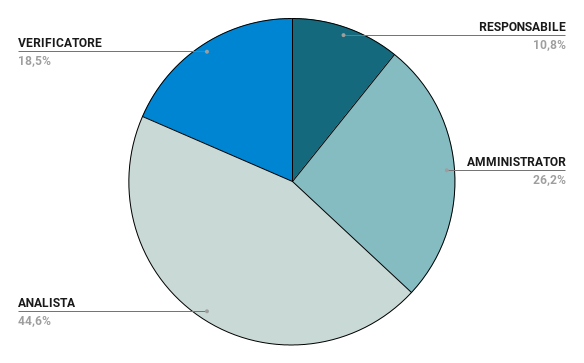
\includegraphics[width=0.8\textwidth]{prev1ruoli.png}
    \caption{Distribuzione dei ruoli primo sprint}
    \label{fig:preventivootarioprimosprint}
\end{figure}


\newpage

\subsubsection{Preventivo economico}

{
\setlength{\tabcolsep}{10pt}
\renewcommand{\arraystretch}{1.5}
\rowcolors{2}{oddrow}{evenrow}
\begin{table}[h]
    \centering
    \begin{tabularx}{\textwidth}{| l | l | l | X |}
        \hline
        \rowcolor{headerrow} \textbf{\textcolor{white}{Ruolo}} & \textbf{\textcolor{white}{Costo orario}} & \textbf{\textcolor{white}{Ore impiegate}} & \textbf{\textcolor{white}{Costo €}} \\
        \hline
        Responsabile & 30 & 7 & 210\\
        \hline
        Amministratore & 20 & 17  & 340\\
        \hline
        Progettista& 25 & 0  & 0\\
        \hline
        Analista & 25 & 29  & 725\\
        \hline
        Programmatore & 15 & 0  & 0\\
        \hline
        Verificatore & 15 & 12  & 180\\
        \hline
        \cellcolor{headerrow} \textbf{\textcolor{white}{Totale}} &  &  & \textbf{1455}\\
        \hline
        \cellcolor{headerrow} \textbf{\textcolor{white}{Rimanente}} &  &  & \textbf{11530}\\
        \hline
    \end{tabularx}
    \caption{Preventivo economico primo sprint}
    \label{tab:preventivocostiprimosprint}
\end{table}
}

\begin{figure}[h!]
    \centering
    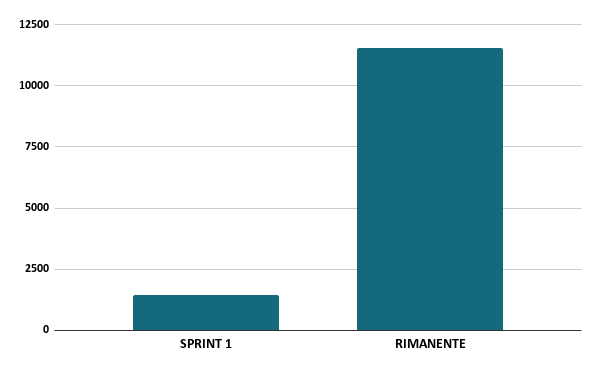
\includegraphics[width=\textwidth]{prev1costo.png}
    \caption{Costo preventivato primo sprint e rimanente}
    \label{fig:preventivocostoprimosprint}
\end{figure}


\newpage


\subsection{Secondo sprint: 2023/11/20 - 2023/12/03}

\subsubsection{Preventivo orario}

{
\setlength{\tabcolsep}{10pt}
\renewcommand{\arraystretch}{1.5}
\rowcolors{2}{oddrow}{evenrow}
\begin{table}[h!]
    \centering
    \begin{tabularx}{\textwidth}{| l | c | c | c | c | c | c | X |}
        \hline
        \rowcolor{headerrow} \textbf{\textcolor{white}{Membro}} & \textbf{\textcolor{white}{R.}} & \textbf{\textcolor{white}{Am.}} & \textbf{\textcolor{white}{Pj.}} & \textbf{\textcolor{white}{An.}} & \textbf{\textcolor{white}{Pg.}} & \textbf{\textcolor{white}{V.}} & \textbf{\textcolor{white}{Totale}} \\
        \hline
        Andrea Cecchin & - & 3 & 3 & - & 3 & - & \textbf{9} \\
        \hline
        Marco Dolzan & - &  & - & 2 & 3 & 4 & \textbf{9} \\
        \hline
        Francesco Ferraioli & - & - & 2 & 5 & - & 2 & \textbf{9} \\
        \hline  
        Francesco Giacomuzzo & 7 & - & - & - & - & 2 & \textbf{9} \\
        \hline
        Leonardo Lago & - & 3 & 3 & - & - & 4 & \textbf{10} \\
        \hline
        Giovanni Menon & - & - & 1 & 5 & 4 & - & \textbf{10} \\
        \hline
        Anna Nordio & - & 2 & - & 5 & 2 & - & \textbf{9} \\
        \hline
    \cellcolor{headerrow} \textbf{\textcolor{white}{Totale}} & \textbf{7} & \textbf{8} & \textbf{9} & \textbf{17} & \textbf{12} & \textbf{12} & \textbf{65} \\
        \hline
    \end{tabularx} 
    \caption{Preventivo orario secondo sprint}
    \label{tab:preventivoorariosecondosprint}
\end{table}
}

\begin{figure}[h!]
    \centering
    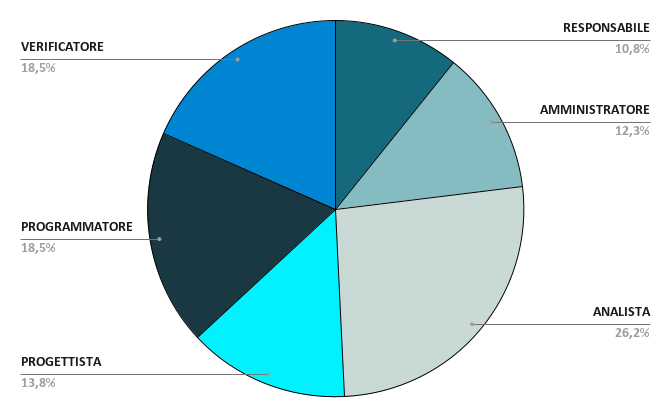
\includegraphics[width=0.8\textwidth]{prev2ruoli.png}
    \caption{Distribuzione dei ruoli secondo sprint}
    \label{fig:preventivootariosecondosprint}
\end{figure}


\newpage
\subsubsection{Preventivo economico}

{
\setlength{\tabcolsep}{10pt}
\renewcommand{\arraystretch}{1.5}
\rowcolors{2}{oddrow}{evenrow}
\begin{table}[h]
    \centering
    \begin{tabularx}{\textwidth}{| l | l | l | X |}
        \hline
        \rowcolor{headerrow} \textbf{\textcolor{white}{Ruolo}} & \textbf{\textcolor{white}{Costo orario}} & \textbf{\textcolor{white}{Ore impiegate}} & \textbf{\textcolor{white}{Costo €}} \\
        \hline
        Responsabile & 30 & 7 & 210\\
        \hline
        Amministratore & 20 & 8 & 160\\
        \hline
        Progettista& 25 & 9  & 225\\
        \hline
        Analista & 25 & 17  & 425\\
        \hline
        Programmatore & 15 & 12 & 180\\
        \hline
        Verificatore & 15 & 12  & 180\\
        \hline
        \cellcolor{headerrow} \textbf{\textcolor{white}{Totale}} &  &  & \textbf{1380}\\
        \hline
        \cellcolor{headerrow} \textbf{\textcolor{white}{Rimanente}} &  &  & \textbf{10240}\\
        \hline
    \end{tabularx}
    \caption{Preventivo economico secondo sprint}
    \label{tab:preventivocostisecondosprint}
\end{table}
}

\begin{figure}[h!]
    \centering
    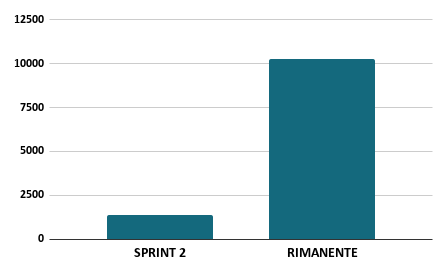
\includegraphics[width=\textwidth]{prev2costo.png}
    \caption{Costo preventivato secondo sprint e rimanente}
    \label{fig:preventivocostosecondosprint}
\end{figure}


\newpage
\subsection{Terzo sprint}
\subsubsection{Preventivo orario}
{
\setlength{\tabcolsep}{10pt}
\renewcommand{\arraystretch}{1.5}
\rowcolors{2}{oddrow}{evenrow}
\begin{table}[h!]
    \centering
    \begin{tabularx}{\textwidth}{| l | c | c | c | c | c | c | X |}
        \hline
        \rowcolor{headerrow} \textbf{\textcolor{white}{Membro}} & \textbf{\textcolor{white}{R.}} & \textbf{\textcolor{white}{Am.}} & \textbf{\textcolor{white}{Pj.}} & \textbf{\textcolor{white}{An.}} & \textbf{\textcolor{white}{Pg.}} & \textbf{\textcolor{white}{V.}} & \textbf{\textcolor{white}{Totale}} \\
        \hline
        Andrea Cecchin & - & 1 & - & - & 4 & 4 & \textbf{9} \\
        \hline
        Marco Dolzan & - & 5 & 2 & - & 2 & - & \textbf{9} \\
        \hline
        Francesco Ferraioli & - & - & - & 4 & 3 & 3 & \textbf{10} \\
        \hline  
        Francesco Giacomuzzo & - & - & 2 & 3 & - & 4 & \textbf{9} \\
        \hline
        Leonardo Lago & 7 & - & - & 2 & - & - & \textbf{9} \\
        \hline
        Giovanni Menon & - & 4 & - & 2 & 4 & - & \textbf{10} \\
        \hline
        Anna Nordio & - & - & 2 & 5 & 3 & - & \textbf{10} \\
        \hline
    \cellcolor{headerrow} \textbf{\textcolor{white}{Totale}} & \textbf{7} & \textbf{10} & \textbf{6} & \textbf{16} & \textbf{16} & \textbf{11} & \textbf{66} \\
        \hline
    \end{tabularx} 
    \caption{Preventivo orario terzo sprint}
    \label{tab:preventivoorarioterzosprint}
\end{table}
}

\begin{figure}[h!]
    \centering
    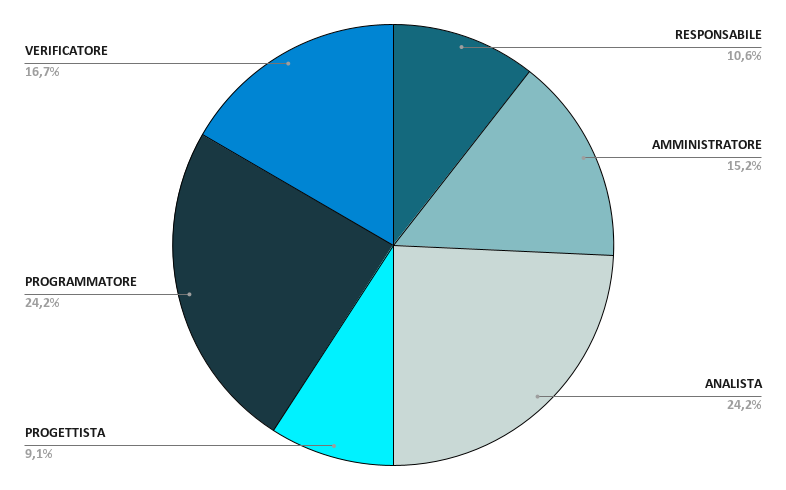
\includegraphics[width=0.9\textwidth]{prev3ruoli.png}
    \caption{Distribuzione dei ruoli terzo sprint}
    \label{fig:preventivootarioterzosprint}
\end{figure}

\subsubsection{Preventivo economico}
{
\setlength{\tabcolsep}{10pt}
\renewcommand{\arraystretch}{1.5}
\rowcolors{2}{oddrow}{evenrow}
\begin{table}[h]
    \centering
    \begin{tabularx}{\textwidth}{| l | l | l | X |}
        \hline
        \rowcolor{headerrow} \textbf{\textcolor{white}{Ruolo}} & \textbf{\textcolor{white}{Costo orario}} & \textbf{\textcolor{white}{Ore impiegate}} & \textbf{\textcolor{white}{Costo €}} \\
        \hline
        Responsabile & 30 & 7 & 210\\
        \hline
        Amministratore & 20 & 10 & 200\\
        \hline
        Progettista& 25 & 6 & 150\\
        \hline
        Analista & 25 & 16 & 400\\
        \hline
        Programmatore & 15 & 16 & 240\\
        \hline
        Verificatore & 15 & 11 & 165\\
        \hline
        \cellcolor{headerrow} \textbf{\textcolor{white}{Totale}} &  &  & \textbf{1365}\\
        \hline
        \cellcolor{headerrow} \textbf{\textcolor{white}{Rimanente}} &  &  & \textbf{8920}\\
        \hline
    \end{tabularx}
    \caption{Preventivo economico terzo sprint}
    \label{tab:preventivocostiterzosprint}
\end{table}
}

\begin{figure}[h!]
    \centering
    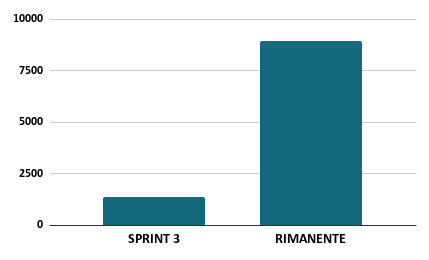
\includegraphics[width=0.9\textwidth]{prev3costo.png}
    \caption{Costo preventivato terzo sprint e rimanente}
    \label{fig:preventivocostoterzosprint}
\end{figure}

\section{Product Baseline}

\newpage